\chapter{Transistores}

En este capítulo se abordará el transistor de unión bipolar (BJT por sus siglas en inglés). Un transistor también está compuesto de material semiconductor, sin embargo no forma parte del capítulo \ref{chpt_introduccion} debido a que no es parte de la introducción necesaria para abordar el documento. 

Antes de progresar debe asegurarse de tener presente el concepto de campo eléctrico. Si desea realizar una revisión conceptual sobre este tema puede leer los capítulos relacionados a electrostática del libro \citetitle{f2elio} --- \cite{f2elio}.

\section{Introducción al Transistor Bipolar}

Un transistor de unión bipolar (BJT) es un dispositivo semiconductor que está compuesto por tres regiones dopadas, como se ilustra en la figura \ref{fig_ilustracion_bjt}. Existen dos tipos principales, \emph{npn} y \emph{pnp} según se haya dopado en cada región. Tal y como es representado, cada región tiene su propio nombre y no son intercambiables (cosa que se fundamentará más adelante).

\begin{figure}[!ht]
  \centering
    \begin{subfigure}[b]{0.7\textwidth}
    \centering
    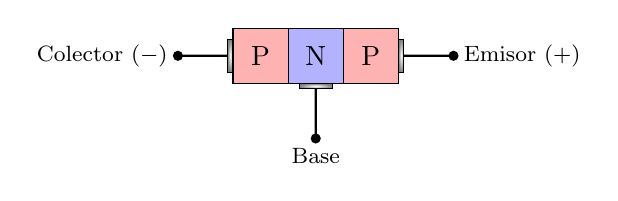
\begin{tikzpicture}[scale=0.7]
      \draw[fill=red!30] (0,0) rectangle node{P} (1,1);
      \draw[fill=blue!30] (1,0) rectangle node{N} (2,1);
      \draw[fill=red!30] (2,0) rectangle node{P} (3,1);
      \filldraw[thick] (-0.1,0.5) -- (-1,0.5) circle (2pt) node[left, font=\footnotesize] {Colector $(-)$};
      \filldraw[thick] (3.1,0.5) -- (4,0.5) circle (2pt) node[right, font=\footnotesize] {Emisor $(+)$};
      \filldraw[thick] (1.5,-0.1) -- (1.5,-1) circle (2pt) node[below, font=\footnotesize] {Base};
      \shadedraw[color=black,fill=gray,inner color=white,outer color=gray] (-0.1,0.2) rectangle (0,0.8);
      \shadedraw[color=black,fill=gray,inner color=white,outer color=gray] (3,0.2) rectangle (3.1,0.8);
      \shadedraw[color=black,fill=gray,inner color=white,outer color=gray] (1.2,-0.1) rectangle (1.8,0);
    \end{tikzpicture}
    \caption{Transistor PNP.}
  \end{subfigure}

  \vspace{5mm}

  \begin{subfigure}[b]{0.7\textwidth}
    \centering
    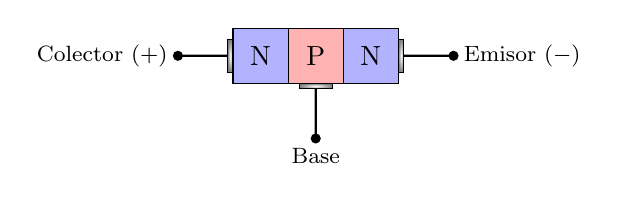
\begin{tikzpicture}[scale=0.7]
      \draw[fill=blue!30] (0,0) rectangle node{N} (1,1);
      \draw[fill=red!30] (1,0) rectangle node{P} (2,1);
      \draw[fill=blue!30] (2,0) rectangle node{N} (3,1);
      \filldraw[thick] (-0.1,0.5) -- (-1,0.5) circle (2pt) node[left, font=\footnotesize] {Colector $(+)$};
      \filldraw[thick] (3.1,0.5) -- (4,0.5) circle (2pt) node[right, font=\footnotesize] {Emisor $(-)$};
      \filldraw[thick] (1.5,-0.1) -- (1.5,-1) circle (2pt) node[below, font=\footnotesize] {Base};
      \shadedraw[color=black,fill=gray,inner color=white,outer color=gray] (-0.1,0.2) rectangle (0,0.8);
      \shadedraw[color=black,fill=gray,inner color=white,outer color=gray] (3,0.2) rectangle (3.1,0.8);
      \shadedraw[color=black,fill=gray,inner color=white,outer color=gray] (1.2,-0.1) rectangle (1.8,0);
    \end{tikzpicture}
    \caption{Transistor NPN.}
  \end{subfigure}
  \caption{Esquema ilustrativo de transistores BJT.}
  \label{fig_ilustracion_bjt}

  \caption{Esquema ilustrativo de transistores BJT.}
  \label{fig_ilustracion_bjt}
\end{figure}

Todas las ilustraciones, como la de la figura \ref{fig_ilustracion_bjt} presentan un defecto estético y didáctico. El hecho de dibujar las tres regiones de igual tamaño y sin distinción puede prestar a una confusión lógica y de compresión importante. En la realidad, como se explicó brevemente en el capítulo \ref{chpt_introduccion} el silicio debe ser dopado para formar material semiconductor tipo \emph{n} (usando Fósforo por ejemplo) y tipo \emph{p} (usando Boro por ejemplo). Pero en ningún caso se habló sobre cuánto Boro o cuanto Fósforo es suficiente o necesario para considerar dopado al semiconductor.

El motivo esencial de omitir la proporción de dopaje durante el estudio del diodo es debido a que no aporta mucho al análisis eléctrico. Sin embargo el diodo (como primera aproximación) es un poco más inofensivo en dicho aspecto, ya que no influye la proporción de dopaje y el tamaño de las regiones dopadas para comprender su funcionamiento. Sin embargo en el transistor la historia cambia un poco. Aquí, Carl, necesariamente deberá detallar cómo es la dimensión física de cada región y qué tan dopada está cada una, ya que esto es lo que hace que existan tres terminales denominadas ``emisor'', ``base'' y ``colector''.

\paragraph{La pregunta sobre los polos del transistor} Estudiando sobre semiconductores, Luis se encontró con estos dispositivos llamados transistores. Como había comprendido el funcionamiento del diodo pensó que el transistor sería casi análogo, pero le tomó un instante encontrar defectos en las explicaciones superficiales. Cuando Luis observó la representación de la figura \ref{fig_ilustracion_bjt} pensó ``¿Por qué no puedo intercambiar el emisor y el colector? ¿Qué hace que sean diferentes?''. 

\paragraph{El mito de los dos diodos y la barrera invisible} Usualmente, un transistor se explica utilizando una analogía que consiste en pensar el transistor como dos diodos en oposición. Si bien esto puede ``dar una idea'' sobre su comportamiento, no es una buena forma de adentrarse al tema. Vea lo que sucede cuando Luis dibuja en la pizarra el esquema mental: un transistor NPN conectado a una batería de \qty{12}{\volt} entre colector (positivo) y emisor (negativo) como muestra la figura \ref{fig_npn_no_polarizado}. Observe que el terminal positivo roba electrones del colector, dejando iones positivos cerca de la unión. 
\begin{figure}[!ht]
  \centering
  \begin{circuitikz}[scale=0.7]
  \draw[fill=blue!30] (0,0) rectangle node{N} (1,1);
  \draw[fill=red!30] (1,0) rectangle node{P} (2,1);
  \draw[fill=blue!30] (2,0) rectangle node{N} (3,1);
  \filldraw[thick] (-0.1,0.5) -- (-1,0.5) coordinate (E) node[below,font=\footnotesize]{E};
  \filldraw[thick] (3.1,0.5) -- (4,0.5) coordinate(C) node[below,font=\footnotesize]{C};
  \filldraw[thick] (1.5,-0.1) -- (1.5,-1) circle (2pt) node[below, font=\footnotesize] {B};
  \shadedraw[color=black,fill=gray,inner color=white,outer color=gray] (-0.1,0.2) rectangle (0,0.8);
  \shadedraw[color=black,fill=gray,inner color=white,outer color=gray] (3,0.2) rectangle (3.1,0.8);
  \shadedraw[color=black,fill=gray,inner color=white,outer color=gray] (1.2,-0.1) rectangle (1.8,0);
  \draw (E) to[short,*-] (-1,2) to[battery,invert,l={\(V_s=\qty{12}{\volt}\)}] (4,2) to[short,-*] (C);
\end{circuitikz}

  \caption{}
  \label{fig_npn_no_polarizado}
\end{figure}

``Si el colector es tipo N y está a \qty{12}{\volt}, sus electrones libres son arrastrados por el positivo de la batería'', razona Luis, intentando unir los conceptos. ``Por el otro lado, el emisor también es N, así que el negativo de la batería empuja sus electrones hacia la base tipo P. Pero la base está llena de huecos... que son, viéndolo así, espacios vacíos. Si esta base está desconectada, los electrones del emisor que llegan ahí se quedan estancados, sin un circuito por donde escapar. Entonces, la zona P actúa simplemente como un aislante pasivo que separa dos regiones con carga... ¿¡Todo este componente no es más que un solo capacitor complicado!?''.

Carl sonríe y niega lentamente con la cabeza. ``Es un razonamiento perfectamente lógico si estuviéramos conectando componentes discretos, pero ahí radica la trampa. Estás imaginando el material tipo P como un simple dieléctrico y tratando a las regiones N como placas de metal. Pensarlo como un capacitor, o incluso como dos diodos soldados por sus ánodos, es un callejón sin salida. En la realidad, el secreto para que los electrones atraviesen esa barrera reside en un delicado equilibrio de dopaje y en un diseño físico extremo''.

\paragraph{Las dos zonas de deplexión}
Carl toma una tiza y dibuja el interior del transistor. Le señala a Luis que, al haber tres bloques, existen \emph{dos} zonas de deplexión: la unión Base-Emisor y la unión Base-Colector, como se representa en la figura \ref{fig_zona_de_deplexión}. 

\begin{figure}[!ht]
  \centering
  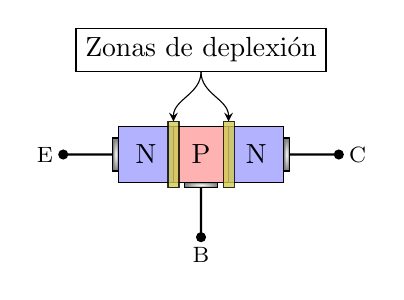
\begin{tikzpicture}[scale=0.7,>=stealth]
  \draw[fill=blue!30] (0,0) rectangle node{N} (1,1);
  \draw[fill=red!30] (1,0) rectangle node{P} (2,1);
  \draw[fill=blue!30] (2,0) rectangle node{N} (3,1);
  \filldraw[thick] (-0.1,0.5) -- (-1,0.5) circle (2pt) node[left, font=\footnotesize] {E};
  \filldraw[thick] (3.1,0.5) -- (4,0.5) circle (2pt) node[right, font=\footnotesize] {C};
  \filldraw[thick] (1.5,-0.1) -- (1.5,-1) circle (2pt) node[below, font=\footnotesize] {B};
  \shadedraw[color=black,fill=gray,inner color=white,outer color=gray] (-0.1,0.2) rectangle (0,0.8);
  \shadedraw[color=black,fill=gray,inner color=white,outer color=gray] (3,0.2) rectangle (3.1,0.8);
  \shadedraw[color=black,fill=gray,inner color=white,outer color=gray] (1.2,-0.1) rectangle (1.8,0);
  \draw[fill=yellow!60!gray,opacity=0.8] (0.9,-0.1) rectangle ++(.2,1.2);
  \draw[fill=yellow!60!gray,opacity=0.8] (1.9,-0.1) rectangle ++(.2,1.2);
  \node[draw, above] (T) at (1.5,2) {Zonas de deplexión};
  \draw[->] (T.south) to[out=270,in=90] (1,1.1);
  \draw[->] (T.south) to[out=270,in=90] (2,1.1);
\end{tikzpicture}

  \caption{Zonas de deplexión en un transistor.}
  \label{fig_zona_de_deplexión}
\end{figure}

Con los \qty{12}{\volt} en el colector y el emisor a tierra (y la base desconectada como se representó en la figura \ref{fig_npn_no_polarizado}), la unión Base-Colector y la unión Base-Emisor sufren un pequeño desplazamiento de cargas.

\paragraph{La trampa de la neutralidad y la base flotante} Carl le transmite un gesto de tranquilidad a Luis. ``Es normal que resulte confuso, pero recuerda siempre los fundamentos que vimos en los diodos: los materiales tipo \emph{p} y tipo \emph{n} son, en su origen, eléctricamente neutros. Esto se debe a que, aunque tengan huecos o electrones libres, el átomo dopante que aporta ese electrón o hueco extra también tiene un protón correspondiente en su núcleo. Todo está balanceado. Solo cuando los electrones se desplazan —por ejemplo, al conectar una batería— es que dejas atrás iones fijos positivos o negativos''. A lo que Luis responde: ``¿Pero y qué sucede con la base desconectada?''.

``Como tienes una zona de deplexión en las interfaces de las zonas \emph{n} y \emph{p}, se crea un campo eléctrico interno que se opone al flujo de electrones'', explica Carl. ``Pero tu batería de \qty{12}{\volt} aplica una gran diferencia de potencial sobre todo el conjunto. La unión Base-Colector absorbe casi todo el impacto y se ensancha, mientras que la Base-Emisor apenas se altera. Esto provoca que la base adquiera un potencial flotante, un poco mayor al polo negativo de la batería. Es decir, su potencial no es cero''. 

Carl hace una pausa y, respondiendo a la duda del equivalente que planteó Luis anteriormente, concluye: ``Así que, complementando tu idea, un transistor con la base desconectada no sería un solo capacitor... más bien se comporta como \emph{dos} capacitores conectados en serie. ¿Súper loco, verdad?''.

\paragraph{Conexión de la base}
``¿Qué pasa si ahora le aplicamos \qty{0.7}{\volt} a la base respecto al emisor?'', pregunta Carl. 

Piense un segundo sobre esta pregunta. Si observa el esquema de la figura \ref{fig_npn_no_polarizado} y añade una fuente de \qty{0.7}{\volt} en la base, ¿qué camino seguirán las cargas? La unión Base-Emisor se comporta como un diodo convencional, por lo que es seguro afirmar que fluirán cargas desde el emisor hacia la base. Pero, ¿qué sucede con el colector?

\paragraph{El diseño físico de un transistor} Carl explica que, si el transistor fuera perfectamente simétrico, la corriente simplemente fluiría hacia la base o se repartiría sin un propósito claro. Sin embargo, en la realidad un transistor no se comporta de esta manera; su principal característica es que la corriente que sale por el terminal de la base es ínfima comparada con la que llega al colector. ``¿Por qué ocurre esto?'', interrumpe Luis, intrigado.

Esto se debe a que el transistor no es un par de diodos ni tampoco un bloque \emph{NPN} simétrico. Su diseño físico real, representado en la figura \ref{fig_npn_representacion_real}, revela proporciones y niveles de dopaje muy específicos. Observe que no solo los tamaños del emisor, base y colector son diferentes, sino que la densidad de portadores también cambia en cada región. El emisor está fuertemente dopado (es decir, es un material con una enorme cantidad de electrones libres agregados). El colector, aunque es la región de mayor tamaño para disipar el calor, tiene un dopaje moderado. Finalmente, la base es físicamente la región más estrecha y está dopada de forma muy débil. Esta asimetría es la clave para que los electrones del emisor saturen la base y, en su gran mayoría, terminen saltando hacia el colector.

\begin{figure}[!ht]
  \centering
  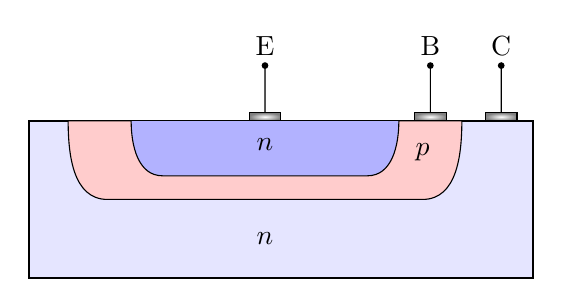
\begin{tikzpicture}
  \draw[fill] (2.1,1) -- ++(0,0.7) circle (1pt) node[above]{B};
  \draw[fill] (0,1) -- ++(0,0.7) circle (1pt) node[above]{E};
  \draw[fill] (3,1) -- ++(0,0.7) circle (1pt) node[above]{C};
  \shadedraw[color=black,fill=gray,inner color=white,outer color=gray] (1.9,1) rectangle (2.3,1.1);
  \shadedraw[color=black,fill=gray,inner color=white,outer color=gray] (-.2,1) rectangle (.2,1.1);
  \shadedraw[color=black,fill=gray,inner color=white,outer color=gray] (2.8,1) rectangle (3.2,1.1);
  \draw[fill=blue!10,thick] (-3,-1) rectangle (3.4,1);
  \draw[fill=blue!30] (-2,0.2) rectangle (2,1);
  \draw[fill=red!20] (-2.5,1) to[out=270,in=180]
    (-2,0) -- (2,0) to[out=0,in=270]
    (2.5,1) -- (1.7,1) to[out=270,in=0]
    (1.3,0.3) -- (-1.3,0.3) to[out=180,in=270] 
    (-1.7,1) -- cycle;
  \node at (0,-.5) {\(n\)};
  \node at (0,.7) {\(n\)};
  \node at (2,.6) {\(p\)};
\end{tikzpicture}

  \caption{Esquema realista del diseño físico y proporciones de un transistor.}
  \label{fig_npn_representacion_real}
\end{figure}

Volviendo al concepto de la barrera de \qty{0.7}{\volt}, Luis analiza la situación: ``Entonces, al superar la barrera de potencial del silicio, la unión Base-Emisor se polariza en directa. Su zona de deplexión se reduce dramáticamente y el emisor, que está fuertemente dopado, inyecta una cantidad masiva de electrones libres hacia la base''.

``¡Exacto! Y aquí es donde el diseño físico rompe las reglas convencionales'', asiente Carl con una sonrisa. ``La base tiene huecos, sí, pero el fabricante la hace \emph{extremadamente delgada} (apenas unos micrómetros) y la dopa \emph{muy débilmente}. Cuando esa avalancha de electrones ingresa a la base, hay tan pocos huecos disponibles que solo alrededor del 1\% de los electrones logra chocar, recombinarse y salir por el cable de la base''.

Carl dibuja flechas gruesas cruzando la región central. ``El 99\% restante de los electrones entra con tanta energía cinética que atraviesa la minúscula base sin encontrar un solo hueco para recombinarse. Antes de que pierdan impulso, se asoman al abismo: la enorme zona de deplexión de la unión Base-Colector''.

Luis, visualizando el panorama completo, concluye: ``Claro... Esa unión estaba en inversa para bloquear a los huecos de la base, pero para los electrones libres que vienen lanzados desde el emisor, ¡ese campo eléctrico actúa como un acelerador directo hacia el colector!''.

``¡Precisamente!'', exclama Carl. ``Esa tensión de \qty{12}{\volt} mantiene un campo eléctrico muy intenso en la zona de deplexión del colector. Cuando los electrones sobreviven al cruce de la base y tocan el borde de esa región, el campo eléctrico los captura y los arrastra con gran fuerza hacia el terminal positivo de la batería, conformando la corriente principal del circuito''.

\paragraph{Visualización real de un BJT} Para finalizar la idea de introducción al transistor, observe el transistor fotografiado bajo un microscópio en la figura \ref{fig_bjt_under_microscope} capturada por \cite{article_transistors}.

\begin{figure}[!ht]
  \centering
  \includegraphics[height=8cm]{chapters/01_capitulo/media/bin/bjt_under_microscope.png}
  \caption{Transistor de unión bipolar capturado bajo el microscópio electrónico.}
  \label{fig_bjt_under_microscope}
\end{figure}

La figura \ref{fig_bjt_under_microscope} demuestra el formato físico de un transistor BJT. Para poder comprender la imagen se dará una breve explicación de qué se está visualizando. Las micrografías obtenidas por Microscopía Electrónica de Barrido (MEB) (imágenes capturadas con un microscópio electrónico) revelan la naturaleza tridimensional del transistor, caracterizada por tres escalones verticales bien definidos. Estos desniveles geométricos corresponden a surcos de aislamiento (\textit{trench isolation}) grabados a diferentes profundidades críticas en la oblea de silicio: el aislamiento del emisor ($\ge 0.5\,\mu\text{m}$), el de la base ($\ge 1.5\,\mu\text{m}$) y el del colector ($\ge 1.0\,\mu\text{m}$). La implementación de estas barreras físicas, posteriormente rellenadas con material dieléctrico, es fundamental en la arquitectura microelectrónica para confinar portadores y prevenir interferencias eléctricas o cortocircuitos entre los terminales de transistores adyacentes que coexisten en el mismo sustrato. 

La inclusión de la figura \ref{fig_bjt_under_microscope} es para que observe que físicamente las regiones de emisor, colector y base son de diferentes tamaños y tienen diferentes propósitos, como ya se explicó anteriormente.

\paragraph{¿El colector como emisor?} Para dar una respuesta concluyente a la pregunta inicial: tras analizar el diseño interno, resulta evidente que el transistor es físicamente asimétrico. Cada región tiene un dopaje y un volumen específicos, por lo que emisor y colector no son intercambiables. Sin embargo, ¿qué sucede si conectamos el componente al revés, invirtiendo estos dos terminales? Técnicamente, el dispositivo operará en lo que se conoce como \emph{región activa inversa}. El transistor funcionará, pero de manera sumamente ineficiente. Al obligar al gran colector (débilmente dopado) a emitir electrones y al minúsculo emisor a intentar recolectarlos, la ganancia de corriente se desploma. Peor aún, la unión Base-Emisor no está diseñada para soportar altas tensiones en inversa, por lo que el componente podría dañarse. En resumen, conectarlo al revés es desperdiciar por completo la genialidad y precisión de su diseño físico.



\section{Nomenclatura y Variables de Circuito}
\label{sec_transistor_nomenclatura}

Ahora que comprende el intrincado diseño físico del transistor, es momento de abstraer su funcionamiento. Un transistor de unión bipolar (BJT) actúa, fundamentalmente, como una válvula controlada por corriente. La gran ventaja de este componente reside en que una corriente minúscula inyectada en la base tiene la capacidad de controlar una avalancha de electrones mucho mayor que fluye desde el emisor hacia el colector. 

Siempre recuerde que la corriente convencional es opuesta a la dirección en la que fluyen los electrones. De esto se trata con detalle en el libro \citetitle{f2elio} de \cite{f2elio}. Sin embargo es conveniente realizar el análisis del transistor usando el flujo de electrones ya que la explicación a nivel atómico lo requiere. Pero luego en el análisis a nivel de circuito se suele emplear la corriente convencional asumiendo que se comprende su funcionamiento electrónico.

Para trasladar esta realidad física al análisis y diseño de redes eléctricas, se emplea una simbología estandarizada, representada en la figura \ref{fig_nomenclatura}.

\begin{figure}[!ht]
  \centering
  \begin{subfigure}[b]{0.4\textwidth}
    \centering
    \begin{circuitikz}
      \draw (0,0) node[npn](Q){};
      \node[font=\footnotesize,left] at (Q.B) {Base};
      \node[font=\footnotesize,above] at (Q.C) {Colector};
      \node[font=\footnotesize,below] at (Q.E) {Emisor};
    \end{circuitikz}
    \caption{Transistor NPN.}
    \label{sfig_npn_symbol}
  \end{subfigure}
  \begin{subfigure}[b]{0.4\textwidth}
    \centering
    \begin{circuitikz}
      \draw (0,0) node[pnp](Q){};
      \node[font=\footnotesize,left] at (Q.B) {Base};
      \node[font=\footnotesize,below] at (Q.C) {Colector};
      \node[font=\footnotesize,above] at (Q.E) {Emisor};
    \end{circuitikz}
    \caption{Transistor PNP.}
  \end{subfigure}
  \caption{Tipos de transistores y su simbología.}
  \label{fig_nomenclatura}
\end{figure}

Observe detenidamente la figura \ref{sfig_npn_symbol}, el transistor \emph{npn} tiene una flecha ubicada en el terminal del emisor. Esta flecha no es un mero detalle estético; es una regla mnemotécnica poderosa y una herencia directa de la analogía de los diodos que dedujo anteriormente junto a Luis y Carl. La flecha indica el sentido de la corriente convencional (de positivo a negativo) y apunta siempre desde la región con dopaje P hacia la región con dopaje N.
\begin{itemize}
  \item En el transistor \textit{NPN}, la base es P y el emisor es N. Por ende, la flecha apunta ``hacia afuera''. Si polariza esta ``unión-diodo'' en directa (aplicando \qty{0.7}{\volt} en la base respecto al emisor), se abre el paso para la gran corriente de colector.
  \item En el transistor \textit{PNP}, el emisor es P y la base es N, por lo que la flecha apunta ``hacia adentro''. Opera bajo los mismos principios, pero de forma complementaria: todas las polaridades de tensión y los sentidos de corriente se invierten.
\end{itemize}

Adicionalmente, se suele utilizar el siguiente vocabulario:
\begin{itemize}
  \item Diodo de emisor: es la unión entre la base y el emisor.
  \item Diodo de colector: La unión entre la base y el colector.
\end{itemize}
Con esto en mente, si dice: ``se conecta el diodo emisor en directa y el diodo colector en inversa'' se está diciendo que el diodo emisor-base se ha conectado en polaridad directa y el diodo colector-base se ha conectado en polaridad inversa.

\subsection{Variables Fundamentales del Circuito}

Para el estudio formal del transistor, especialmente durante el análisis en corriente continua (DC), utilizamos un conjunto de variables estandarizadas con letras y subíndices en mayúscula:
\begin{enumerate}
  \item \(V_{CC}\) (o \(V_{EE}\)): Tensión de alimentación de la fuente. Representa la energía principal que abastece a la malla de salida del circuito.
  \item \(I_B, I_C, I_E\): Corrientes de base, colector y emisor, respectivamente. La corriente de base (\(I_B\)) actúa como la señal de control, la del colector (\(I_C\)) es la corriente controlada, y la de emisor es la suma de ambas (\(I_E = I_B + I_C\) por ley de corrientes de Kirchhoff).
  \item \(V_{CE}\): Tensión colector-emisor. Es la caída de potencial a través de los terminales de salida del transistor. Su valor es el indicador definitivo para determinar en qué región está operando el dispositivo (corte, activa o saturación).
  \item \(V_{BE}\): Tensión base-emisor. Es el umbral de encendido. Cuando el transistor opera en la región activa, esta unión se comporta como un diodo polarizado en directa, asumiéndose una caída térmica\footnote{Se dice caída térmica ya que la caída de potencial \(V_{BE}\) depende de la temperatura de operación.} casi constante de \qty{0.7}{\volt} para el silicio.
  \item \(\beta\) (también denotado en las hojas de datos como \(h_{FE}\)): Ganancia estática de corriente en configuración emisor común\footnote{La configuración en \emph{emisor común} es una topología de circuito donde el terminal del emisor se conecta al punto de referencia (comúnmente tierra). Al estar referenciado a tierra, el emisor actúa como un nodo compartido tanto para el lazo de entrada (entre base y emisor) como para el lazo de salida (entre colector y emisor). Es la configuración más utilizada debido a que proporciona una gran amplificación tanto de voltaje como de corriente.}. Representa el factor de multiplicación del transistor, definiendo la relación directa en la región activa: \(I_C = \beta I_B\).

    La ganancia de corriente \(\beta\) es un valor muy importante de un transistor y será muy utilizado en general.
\end{enumerate}

Del ítem 2, observe que se puede obtener una comparación de las corrientes. Dado que el emisor es la fuente de los electrones, es la corriente más grande. La mayor parte del flujo de electrones llega al colector, por lo que la corriente de colector es prácticamente igual a la corriente de emisor. En comparación, la corriente de la base es muy pequeña, a menudo menor que el 1\% de la corriente de colector. Por lo tanto, generalmente la aproximación 
\[
  I_E \approx I_C
\]
se considera válida.

\subsection{Resistencias del Circuito de Polarización}

Un transistor rara vez se conecta directamente a las fuentes de tensión. Para establecer un punto de operación seguro (conocido como punto \(Q\)), se diseña una red de polarización mediante resistencias externas. Es vital mantener la consistencia en su nomenclatura:

\begin{itemize}
  \item \(R_B\) (Resistencia de base): Se coloca en serie con el terminal de entrada. Su función es restringir y fijar la corriente \(I_B\), protegiendo la unión base-emisor de corrientes excesivas que podrían destruirla.
  \item \(R_C\) (Resistencia de colector): Ubicada en la rama principal de salida. No solo limita la corriente máxima \(I_C\), sino que tiene una función crucial en los amplificadores: convierte las variaciones de corriente de colector en variaciones de tensión (\(V_{CE}\)) que pueden ser entregadas a la siguiente etapa del circuito.
  \item \(R_E\) (Resistencia de emisor): Aunque es opcional en los circuitos más elementales, su función principal es proporcionar estabilidad al punto de operación. Genera un efecto de realimentación negativa térmica: si el transistor se calienta y su ganancia (\(\beta\)) aumenta, \(R_E\) frena el incremento descontrolado de la corriente, evitando que el componente se destruya.
\end{itemize}


\section{Tipos de conexión}

Las siguientes son tres formas de conectar un transistor: emisor común (EC), colector común (CC) o base común (BC). Para los fines de este capítulo solo se analizará la conexión EC, ya que es la más utilizada.

\subsection{Emisor común}

En teoría de circuitos se llama lazo a una trayectoria cerrada de corriente dentro del circuito. Por ejemplo la figura \ref{sfig_ej_lazo} representa un lazo que consiste de una resistencia y una fuente de tensión. 

Por otro lado, la figura \ref{sfig_circuito_ec} tiene dos mallas: la malla de la izquierda es la malla de la base y la de la derecha es la malla del colector. En la malla de la base, la fuente \(V_{BB}\) polariza en directa al diodo de emisor con \(R_B\) como resistencia limitadora de corriente. Cambiando \(V_{BB}\) o \(R_B\) se puede cambiar la corriente de base, y por lo tanto cambiar la corriente de colector. En otras palabras, la corriente de la base controla la corriente del colector.

\begin{figure}[!ht]
  \centering
  \begin{subfigure}[t]{0.25\textwidth}
    \centering
    \begin{circuitikz}[scale=0.8,transform shape]
      \draw (0,0) to[battery,invert] (0,3) to[short] (2,3) to[R] (2,0) to[short] (0,0);
    \end{circuitikz}
    \caption{Ejemplo de lazo.}
    \label{sfig_ej_lazo}
  \end{subfigure}
  \hspace{0.5cm}
  \begin{subfigure}[t]{0.6\textwidth}
    \centering
    \begin{circuitikz}[scale=0.8,transform shape]
      \draw (0,0) node[npn](Q){};
      \draw (Q.C) to[short] ++(0,0.5) to[R,l={\(R_C\)}] ++(2.5,0) to[battery,l={\(V_{CC}\)}] ++(0,-3) coordinate(GND) node[ground]{};
      \draw (Q.B) to[R,l_={\(R_B\)}] ++(-3,0) coordinate(tmp) to[battery,l_={\(V_{BB}\)}] (GND -| tmp) node[ground]{};
      \draw (Q.E) -- (GND -| Q.E) node[ground]{};
    \end{circuitikz}
    \caption{Topología de circuito con configuración EC.}
    \label{sfig_circuito_ec}
  \end{subfigure}
  \caption{}
\end{figure}

En la malla de colector, una tensión de fuente \(V_{CC}\) polariza en inversa al diodo de colector a través de \(R_C\). La tensión de alimentación \(V_{CC}\) debe polarizar en inversa el diodo colector, de lo contrario el transistor no funcionará apropiadamente. Dicho de otra manera, el colector debe ser positivo para recolectar los electrones libres.


\section{Curvas Características del Transistor}

Los transistores son dispositivos no lineales. Su comportamiento cambia drásticamente dependiendo de cuánta corriente o voltaje se les inyecte. A diferencia de resistores o componentes lineales, no se los puede definirlo con una sola ecuación simple; más bien se requiere un mapa de su comportamiento. Ese mapa son las curvas características.

A continuación verá que un transistor tiene cuatro regiones importantes. Cada región representa un modo de operación completamente distinto. Dependiendo de lo que se esté diseñando o reparando, se fuerza el componente a trabajar en una región específica.

Para que esta sección no sea extremadamente tediosa, Carl ayudará a Luis a comprender el significado de cada región.

\subsection{Curva característica de entrada}
Observando el circuito de la figura \ref{fig_circuito_em_comm} ¿Qué forma cree que tiene la gráfica de la corriente de base \(I_B\) en función de la tensión base-emisor \(V_{BE}\) (\(I_B(V_{BE})\))? Preguntó Carl. Si recuerda, esta unión se comporta exactamente como un diodo convencional. Entonces la respuesta es inmediata: su gráfica es idéntica a la de un diodo polarizado en directa.
\begin{figure}[!ht]
  \centering
  \begin{circuitikz}[scale=0.8,transform shape]
    \draw (0,0) node[npn](Q){};
    \draw (Q.C) to[short] ++(0,0.5) to[R,l={\(R_C\)}] ++(2.5,0) to[battery,l={\(V_{CC}\)}] ++(0,-3) coordinate(GND) node[ground]{};
    \draw (Q.B) to[R,l_={\(R_B\)}] ++(-3,0) coordinate(tmp) to[battery,l_={\(V_{BB}\)}] (GND -| tmp) node[ground]{};
    \draw (Q.E) -- (GND -| Q.E) node[ground]{};
  \end{circuitikz}
  \caption{Topología de circuito con configuración EC.}
  \label{fig_circuito_em_comm}
\end{figure}

Por lo tanto, podemos aplicar las mismas simplificaciones estudiadas anteriormente en el capítulo \ref{chpt_introduccion}. Al analizar la malla de entrada, la corriente se define por la ley de Ohm:
\[
  I_B = \frac{V_{BB} - V_{BE}}{R_B}
\]
Para el análisis práctico de circuitos, la segunda aproximación del diodo es el equilibrio perfecto entre simplicidad y precisión. Basta con asumir que, una vez encendido el transistor, la barrera de potencial \(V_{BE}\) se mantiene casi constante en aproximadamente \qty{0.7}{\volt}.

\subsection{Curva de colector y regiones de operación}

La verdadera naturaleza del transistor se revela al observar su salida. ``¿A qué llamamos salida?'', interrumpe Luis.

``Llamamos salida a la corriente de colector en función de la tensión colector-emisor'', respondió Carl, y anotó en la pizarra
\[
  I_C(V_{CE}) \quad \text{(Función de salida)}
\]

Para poder estudiar esta función, supongamos que fijamos la corriente de base \(I_B\) en un valor pequeño y constante (por ejemplo, \qty{10}{\micro\ampere}). A continuación, comenzamos a variar la tensión de la fuente del colector y medimos tanto la corriente de colector \(I_C\) como la tensión en los terminales \(V_{CE}\). 

Al trazar estas mediciones, la gráfica resultante no es una línea recta como dictaría una resistencia simple, sino que revela distintas zonas de comportamiento dictadas por el diseño interno del componente.

La figura \ref{fig_curvas_de_colector} representa las curvas para distintas corrientes de base (\qty{10}{\micro\ampere}, \qty{20}{\micro\ampere}, etcétera).

\begin{figure}[!ht]
  \centering
  \begin{tikzpicture}[scale=0.8,>=stealth]
  \draw[->,gray] (-.4,0) -- (8.4,0) node[right,font=\scriptsize]{\(V_{CE}\)};
  \draw[->,gray] (0,-.4) -- (0,8.4) node[above,font=\scriptsize]{\(I_C\) [\unit{\milli\ampere}]};

  \draw[thick,teal!40] (0,0) -- ++(20:.05) to[out=20,in=180] ++(.35,.1) -- 
    node[midway,above,font=\tiny,color=black]{\(I_B=\qty{0}{\ampere}\) (Corriente de base)} ++(7.5,0) to[out=0,in=260] ++(.2,.5) 
    -- ++(.2,1.8);
  \draw[thick,teal!40] (0,0) -- ++(70:.5) to[out=70,in=180] ++(.35,.3) -- 
    node[midway,above,font=\tiny,color=black]{\qty{10}{\micro\ampere}} ++(7.1,0) to[out=0,in=260] ++(.2,.5) 
    -- ++(.2,2);
  \foreach \i [evaluate=\i as \corriente using int(20*\i)] in {1,1.5,2,2.5,3,3.5} {
    \draw[thick,teal!40] (0,0) -- ++(70:\i) to[out=70,in=180] ++(.35,.4) -- 
      node[midway,above,font=\tiny,color=black]{\qty{\corriente}{\micro\ampere}} ++(7.6-\i,0) to[out=0,in=260] ++(.2,.5) 
      -- ++(.2,{\i+1/\i});
  }
  \foreach \i in {1,2,3,4,5,6,7,9,10,11,12,13,14,15}{
    \draw[gray,thin] (.1,0.52*\i+.2) -- (-.1,0.52*\i+.2) node[left,font=\tiny]{\qty{\i}{\milli\ampere}};
  }
  \draw[gray,thin] (1,0) -- (1,-0.1) node[below,font=\tiny]{\qty{1}{\volt}};
  \draw[gray,thin] (7.6,0) -- (7.6,-0.1) node[below,font=\tiny]{\qty{40}{\volt}};
  \draw[gray!50!blue,->] (-2.3,5) node[above,text width=1.5cm,align=center,font=\scriptsize,draw]{Región de saturación} to[out=-90,in=120] (70:4);
  \draw[gray!50!red,->] (10,5) node[above,text width=1.5cm,align=center,font=\scriptsize,draw]{Región de disrupción} to[out=-90,in=60] (8,4);
  \draw[black!50!gray!50!green,->] (3.5,6.5) node[above,text width=1cm,align=center,font=\scriptsize,draw]{Región activa} -- ++(0,-2);
\end{tikzpicture}

  \caption{Conjunto de curvas de colector.}
  \label{fig_curvas_de_colector}
\end{figure}

\paragraph{La región activa}
Si observa la gráfica a medida que \(V_{CE}\) supera un valor mínimo, verá que la curva se vuelve casi completamente horizontal. Es decir, \(I_C\) se mantiene constante aunque sigamos aumentando la tensión entre el colector y el emisor. 

``¿Por qué ocurre esto?'', preguntó Carl. A lo que Luis, recordando la explicación física que antes dedujo, respondió: ``El colector se limita a atrapar los electrones que el emisor logra inyectar a través de la base. La cantidad de electrones disponibles depende única y exclusivamente de la corriente de base \(I_B\). Por más que aumentemos el voltaje \(V_{CE}\) para intentar succionar más corriente, el colector no puede absorber electrones que no existen''. Carl complementó esta explicación, añadiendo que en esta zona plana, conocida como región activa, el transistor actúa como un amplificador perfecto donde la corriente de salida es simplemente un múltiplo de la entrada (\(I_C = \beta I_B\)).

\paragraph{La región de saturación}
¿Qué sucede en la parte inicial de la gráfica, cuando \(V_{CE}\) se acerca a \qty{0}{\volt}? En este punto, la tensión del colector es tan débil que su campo eléctrico pierde la fuerza necesaria para capturar a los electrones que cruzan la base. Al no haber un ``tobogán'' lo suficientemente inclinado para barrerlos, la corriente de colector cae abruptamente hacia cero. A esta pendiente casi vertical se la conoce como región de saturación.

\paragraph{La región de disrupción}
Como regla general, el transistor jamás debe operar en esta región, ya que el resultado es su destrucción casi instantánea. Esta zona crítica se alcanza cuando la tensión $V_{CE}$ se eleva a niveles no soportados por el dispositivo. Al hacerlo, el campo eléctrico en la unión Base-Colector se vuelve tan intenso que acelera a los electrones a velocidades catastróficas. Estos chocan contra la estructura cristalina del silicio y arrancan violentamente a otros electrones de sus enlaces, generando un efecto multiplicador de avalancha. El resultado es una corriente masiva y descontrolada que atraviesa el dispositivo, ignorando por completo cualquier orden dictada por la base, y que termina destruyendo el componente de forma irreversible.

\paragraph{La región de corte}
Si realizamos el experimento forzando \(I_B = 0\) (por ejemplo, desconectando la base), esperaríamos que la corriente de colector fuera exactamente cero. En la gráfica, esto se representa como una curva microscópica pegada al eje horizontal inferior. Esta ínfima circulación se debe a corrientes de fuga térmicas propias de los semiconductores, pero en la inmensa mayoría de las aplicaciones prácticas es tan pequeña que el transistor se considera un interruptor abierto perfecto.

\subsection{Familia de curvas y límites de potencia}
Si repetimos el procedimiento midiendo \(I_C\) para distintos valores fijos de \(I_B\) (\qty{20}{\micro\ampere}, \qty{30}{\micro\ampere}, etc.), obtendremos una familia de curvas. Cada peldaño horizontal superior representa una corriente de colector proporcionalmente mayor. Este conjunto de gráficas es la huella dactilar del transistor y define su ganancia de corriente continua (\(\beta\)).

Sin embargo, el funcionamiento en estas regiones tiene límites físicos ineludibles. Aplicando la ley de las tensiones de Kirchhoff en la malla de salida, la caída de potencial en el dispositivo es:
\[
V_{CE} = V_{CC} - I_C R_C
\]
Y la potencia que el transistor debe disipar en forma de calor es el producto de su tensión y su corriente:
\[
P_D = V_{CE} I_C
\]
Si la combinación de voltaje y corriente genera una potencia (\(P_D\)) que supera la potencia máxima especificada por el fabricante, la temperatura interna excederá rápidamente los \qty{150}{\degreeCelsius} y el cristal de silicio se destruirá por exceso térmico. 

De manera similar, si continuamos aumentando \(V_{CE}\) desproporcionadamente en la gráfica, llegaremos a un muro infranqueable: la \textit{región de disrupción} (o ruptura). Por ello, el diseño de cualquier circuito debe asegurar que el transistor opere siempre dentro de las zonas seguras (activa, corte o saturación), lejos de estos límites destructivos.




\subsection{La recta de carga: el entorno dicta las reglas}

Tras observar la familia de curvas, Carl borra parte de la pizarra para hacer un cambio de perspectiva radical. ``Hasta ahora hemos analizado las curvas características, que representan la identidad o el ADN del transistor. No importa dónde lo conectes, esas curvas dictan de lo que es físicamente capaz de hacer por sí solo'', explica el profesor. ``Sin embargo, cuando lo soldamos a una placa, el transistor ya no manda en solitario''.

Carl dibuja una línea recta superpuesta sobre las curvas de salida del transistor. ``Esta es la \emph{recta de carga}. Y, a diferencia de las curvas que vimos antes, no tiene absolutamente nada que ver con el transistor en sí. Representa a todo el circuito externo que has conectado a sus terminales; específicamente, tu fuente de alimentación y tus resistencias. Es, literalmente, la representación gráfica de las leyes de Kirchhoff impuestas sobre tu circuito''.
\begin{figure}[!ht]
  \centering
  \input{chapters/01_capitulo/media/5_recta_de_carga.tex}
  \caption{Recta de carga del circuito de la figura \ref{fig_circuito_em_comm2}.}
\end{figure}

\paragraph{La matemática detrás de la recta}
Para demostrarlo, Carl plantea la malla de salida de un circuito básico: la energía parte de la fuente \(V_{CC}\), baja por la resistencia \(R_C\), atraviesa el transistor desde el colector hasta el emisor (\(V_{CE}\)) y finalmente llega a tierra como muestra la figura \ref{fig_circuito_em_comm2}.
\begin{figure}[!ht]
  \centering
  \begin{circuitikz}[scale=0.8,transform shape]
    \draw (0,0) node[npn](Q){};
    \node[right] at (Q.center){\(V_{CE}\)};
    \draw (Q.C) to[short] ++(0,0.5) coordinate(tmp) to[R,l={\(R_C=\qty{3}{\kilo\ohm}\)}] ++(2.5,0) to[battery,l={\(V_{CC}=\qty{15}{\volt}\)}] ++(0,-3) coordinate(GND) node[ground]{};
    \draw (Q.B) to[R,l={\(R_B=\qty{497}{\kilo\ohm}\)}] ++(-3,0) coordinate(tmp2) -- (tmp -| tmp2) to[short,-*] (tmp);
    \draw (Q.E) -- (GND -| Q.E) node[ground]{};
  \end{circuitikz}
  \caption{Esquema para representar la recta de carga.}
  \label{fig_circuito_em_comm2}
\end{figure}

Aplicando la ley de las tensiones de Kirchhoff, escribe en la pizarra:
\[
V_{CC} = I_C R_C + V_{CE}
\]
``Si despejamos la corriente de colector (\(I_C\)) para poder graficarla en el eje vertical, en función de la tensión del transistor (\(V_{CE}\)) en el eje horizontal'', continúa Carl, reordenando los términos, ``obtenemos la inconfundible ecuación de una línea recta (\(y = m x + b\))'':
\[
I_C = \left(-\frac{1}{R_C}\right) V_{CE} + \frac{V_{CC}}{R_C}
\]

Luis observa la ecuación y rápidamente deduce los límites físicos de esa recta. ``Claro... el corte en el eje horizontal (el voltaje máximo) sería cuando el transistor está apagado y no pasa corriente, es decir, \(I_C = 0\). Como no hay caída de tensión en la resistencia, todo el voltaje de la fuente cae sobre el transistor. Por lo tanto, \(V_{CE} = V_{CC}\)''.

``¡Exacto! Y el corte en el eje vertical ocurre en el extremo opuesto'', afirma Carl. ``Si imaginamos que el transistor es un cortocircuito perfecto (\(V_{CE} = 0\)), la corriente máxima posible estará limitada únicamente por la fuente y la resistencia externa. Por pura ley de Ohm, el límite superior es \(I_C = \frac{V_{CC}}{R_C}\)''.

\paragraph{La pendiente y el compromiso eléctrico}
``¿Y de qué depende su pendiente?'', se pregunta Luis en voz alta, analizando la fórmula.
    
``Observa el término que acompaña a tu variable'', señala Carl, golpeando la tiza contra el paréntesis de la ecuación. ``La pendiente es \(-\frac{1}{R_C}\). Depende única y exclusivamente de la resistencia de carga que hayas colocado en tu circuito. Si pones una resistencia muy grande, la fracción se hace minúscula y la pendiente se `acuesta', volviéndose casi horizontal. Si pones una resistencia muy chica, la fracción crece y la recta se vuelve mucho más vertical''.

Para cerrar la idea, Carl recurre a una analogía más cotidiana. ``Imagina que vas pedaleando en tu bicicleta. Tú, al igual que el transistor, tienes tu propia `curva' de rendimiento biomecánico: a tal esfuerzo muscular, logras cierta cadencia. Pero la pendiente de la calle y el rozamiento del viento actúan como tu circuito externo, imponiendo sus propias reglas físicas y limitando lo que realmente puedes alcanzar''. 

Carl dibuja un gran punto donde la línea recta corta una de las curvas del transistor como muestra la figura \ref{fig_punto_q}. ``Tu rendimiento real al pedalear es un compromiso entre tu capacidad y las condiciones del entorno. En electrónica ocurre exactamente lo mismo. El único estado eléctrico posible donde el transistor cumple sus propias leyes internas y, al mismo tiempo, respeta el circuito externo al que está conectado, es el punto exacto donde la recta y la curva se cruzan. A este cruce lo llamamos \emph{Punto de Operación} o \emph{Punto Q}''. Observe que el punto Q se posicionará según sea la corriente de base. Como en el circuito de la figura \ref{fig_circuito_em_comm2} la corriente de base es de 
\[
  I_B = \frac{\qty{15}{\volt}}{\qty{500}{\kilo\ohm}}=\qty{30}{\micro\ampere}
\]
entonces el punto Q es la intersección de la recta de carga y la curva del transistor correspondiente a la corriente de base de \qty{30}{\micro\ampere}.

\begin{figure}[!ht]
  \centering
  \begin{tikzpicture}[scale=0.8,>=stealth]
  \draw[->,gray] (-.4,0) -- (8.4,0) node[right,font=\scriptsize]{\(V_{CE}\)};
  \draw[->,gray] (0,-.4) -- (0,5.4) node[above,font=\scriptsize]{\(I_C\) [\unit{\milli\ampere}]};

  \draw[thick,teal!40] (0,0) -- ++(20:.05) to[out=20,in=180] ++(.35,.1) -- 
    node[midway,above,font=\tiny,color=black]{\(I_B=\qty{0}{\ampere}\) (Corriente de base)} ++(7.5,0);
  \draw[thick,teal!40] (0,0) -- ++(70:.5) to[out=70,in=180] ++(.35,.3) -- 
    node[midway,above,font=\tiny,color=black]{\qty{10}{\micro\ampere}} ++(7.1,0);
  \foreach \i [evaluate=\i as \corriente using int(20*\i)] in {1,1.5,2,2.5,3,3.5} {
    \draw[thick,teal!40] (0,0) -- ++(70:\i) to[out=70,in=180] ++(.35,.4) -- 
      node[midway,above,font=\tiny,color=black]{\qty{\corriente}{\micro\ampere}} ++(7.6-\i,0);
  }
  \foreach \i in {1,2,3,4,5,6,7}{
    \draw[gray,thin] (.1,0.52*\i+.2) -- (-.1,0.52*\i+.2) node[left,font=\tiny]{\qty{\i}{\milli\ampere}};
  }
  \draw[gray,thin] (1,0) -- (1,-0.1) node[below,font=\tiny]{\qty{1}{\volt}};
  \draw[gray,thin] (7.6,0) -- (7.6,-0.1) node[below,font=\tiny]{\qty{40}{\volt}};
  \draw[gray!50!blue,->] (-2.3,5) node[above,text width=1.5cm,align=center,font=\scriptsize,draw]{Punto de saturación} to[out=-90,in=120] (-0.1,2.9);
  \draw[gray!50!red,->] (7,2) node[above,fill=white,text width=1.5cm,align=center,font=\scriptsize,draw]{Punto de corte} to[out=-90,in=60] (5.1,0.1);
  \filldraw[very thick] (0,2.8) circle (1pt) -- (5,0) circle (1pt) node[below,font=\small]{\qty{15}{\volt}};
  \filldraw (1.75,1.83) circle (3pt) node[above=.3cm,draw,fill=white]{Q};
\end{tikzpicture}

  \caption{Determinación del punto Q.}
  \label{fig_punto_q}
\end{figure}

Luis asiente, comprendiendo finalmente la filosofía detrás de los esquemas que dibujaba mecánicamente. ``Por eso, al diseñar un circuito desde cero, lo primero que haces no es buscar el transistor...''.

``Así es'', concluye Carl. ``Primero planteas tu recta de carga. Determinas qué corriente necesitas y qué fuente de alimentación tienes, lo que te dará tu pendiente y tus límites. Una vez que estableciste las reglas del entorno, recién entonces buscas en los manuales un transistor cuyas curvas se acomoden bien a la recta que tú ya trazaste''.



\section{Ejercicios para el lector}

Este capítulo es un poco extenso, pero la finalidad es que usted logre identificar cuestiones básicas de un transistor así como poder comprender un circuito básico que contenga transistores.

\subsection{Preguntas teóricas}

\begin{enumerate}
  \item ¿Qué es un transistor de unión bipolar?
  \item ¿Qué tipos de transistores hay?
  \item ¿Por qué un transistor no es lo mismo que dos diodos juntos?
  \item ¿Cuántas zonas de deplexión tiene un transistor?
  \item ¿Por qué un transistor no es un capacitor cuando su base está desconectada?
  \item ¿Por qué el diseño físico y la cantidad de dopaje es importante en el diseño del transistor?
  \item ¿Qué sucede si conecto un transistor al revés?
  \item El transistor de unión bipolar ¿es un dispositivo controlado por tensión o por corriente?
  \item ¿Qué es el parámetro \(\beta\) del transistor?
  \item ¿Qué tensión es la responsable de controlar el flujo de corriente de colector?
  \item ¿Qué significa conectar un transistor en configuración emisor común?
  \item ¿Qué regiones de operación tiene un transistor?
  \item ¿Qué es la curva de carga?
  \item ¿Cómo se obtiene el punto Q?
\end{enumerate}

% Respuestas
% \begin{enumerate}
%   \item Es un dispositivo de material semiconductor conformado de tres regiones dopadas. 
%   \item Existen dos tipos: PNP y NPN
%   \item No es lo mismo que dos diodos juntos porque en un transistor no son todas sus regiones iguales. La base es muy estrecha y debilmente dopada, el colector es más grande y ligeramente dopado y el emisor es fuertemente dopado, pero más pequeño que el colector. Este diseño hace que sea posible el pasaje de cargas al colector cuando se satura la base. En un par de diodos esto nunca pasaría.
%   \item El transistor tiene dos zonas de deplexión.
%   \item El transistor no es un capacitor cuando la base está desconectada porque existen dos zonas de deplexión. Esto hace que cuando se conecte el colector al terminal positivo de una fuente de tensión y el emisor al terminal negativo, se desplacen las cargas y las zonas de deplexión, pero no se conduzca corriente eléctrica. La zona del colector se ensancha enormemente. La zona del emisor se desplaza hacia la base. Esto provoca un corrimiento de potencial de la base y consecuentemente la base tiene un potencial mayor a cero. Esto implica que no sería equivalente a un solo capacitor sino dos capacitores en serie.
%   \item El diseño físico y la cantidad de dopaje es importante por lo explicado en el inciso 3. Básicamente el transistor se diseña para que cada una de las regiones tenga un propósito específico. El emisor es un acumulador de cargas, la base es un puente o barrera según se polarice entre el emisor y colector. Y por último el colector es un gran recolector de cargas libres.
%   \item Si conecto un transistor al revés técnicamente funcionará, pero no lo hará como debería. Esto significa que su rendimiento será pobre ya que no se está aprovechando el diseño físico de los componentes.
%   \item El transistor es un dispositivo controlado por corriente.
%   \item El parámetro \(\beta\) es un parametro llamado ganancia de corriente del transistor, y se define con la relación \(I_C=\beta I_B\).
%   \item La tensión responsable de controlar \(I_C\) es \(V_{BE}\) (Base-Emisor), ya que de esta tensión depende la cantidad de corriente que circula por el colector. Con un pequeño cambio en \(V_{BE}\) se produce un cambio significativo de \(I_C\).
%   \item Significa conectar el emisor del transistor en GND o la conexión común, de modo que se formen lazos compartidos entre la entrada y la salida.
% \end{enumerate}

